%%%%%%%%%%%%%%%%%%%%%%%%%%%%%%%%%%%%%%%%%
% Beamer Presentation
% LaTeX Template
% Version 1.0 (10/11/12)
%
% This template has been downloaded from:
% http://www.LaTeXTemplates.com
%
% License:
% CC BY-NC-SA 3.0 (http://creativecommons.org/licenses/by-nc-sa/3.0/)
%
%%%%%%%%%%%%%%%%%%%%%%%%%%%%%%%%%%%%%%%%%

%----------------------------------------------------------------------------------------
%	PACKAGES AND THEMES
%----------------------------------------------------------------------------------------

\documentclass{beamer}

\mode<presentation> {

% The Beamer class comes with a number of default slide themes
% which change the colors and layouts of slides. Below this is a list
% of all the themes, uncomment each in turn to see what they look like.

%\usetheme{default}
%\usetheme{AnnArbor}
%\usetheme{Antibes}
%\usetheme{Bergen}
%\usetheme{Berkeley}
%\usetheme{Berlin}
%\usetheme{Boadilla}
%\usetheme{CambridgeUS}
%\usetheme{Copenhagen}
%\usetheme{Darmstadt}
\usetheme{Dresden}
%\usetheme{Frankfurt}
%\usetheme{Goettingen}
%\usetheme{Hannover}
%\usetheme{Ilmenau}
%\usetheme{JuanLesPins}
%\usetheme{Luebeck}
%\usetheme{Madrid}
%\usetheme{Malmoe}
%\usetheme{Marburg}
%\usetheme{Montpellier}
%\usetheme{PaloAlto}
%\usetheme{Pittsburgh}
%\usetheme{Rochester}
%\usetheme{Singapore}
%\usetheme{Szeged}
%\usetheme{Warsaw}

% As well as themes, the Beamer class has a number of color themes
% for any slide theme. Uncomment each of these in turn to see how it
% changes the colors of your current slide theme.

%\usecolortheme{albatross}
%\usecolortheme{beaver}
%\usecolortheme{beetle}
%\usecolortheme{crane}
%\usecolortheme{dolphin}
%\usecolortheme{dove}
%\usecolortheme{fly}
%\usecolortheme{lily}
%\usecolortheme{orchid}
%\usecolortheme{rose}
%\usecolortheme{seagull}
%\usecolortheme{seahorse}
%\usecolortheme{whale}
%\usecolortheme{wolverine}

%\setbeamertemplate{footline} % To remove the footer line in all slides uncomment this line
%\setbeamertemplate{footline}[page number] % To replace the footer line in all slides with a simple slide count uncomment this line

%\setbeamertemplate{navigation symbols}{} % To remove the navigation symbols from the bottom of all slides uncomment this line
}

\usepackage{graphicx} % Allows including images
\usepackage{booktabs} % Allows the use of \toprule, \midrule and \bottomrule in 
%tables
\usepackage{listings}
\usepackage{hyperref}

%----------------------------------------------------------------------------------------
%	TITLE PAGE
%----------------------------------------------------------------------------------------

\title[Lecture 3]{Advanced R Programming - Lecture 3} % The short title 
%appears at the bottom of every slide, the full title is only on the title page

\author{Leif Jonsson} % Your name
\institute[STIMA LiU] % Your institution as it will appear on the bottom of 
%every 
%slide, may be shorthand to save space
{
Link\"{o}ping University \\ % Your institution for the title page
\medskip
\textit{leif.jonsson@ericsson.com\\leif.r.jonsson@liu.se} % Your email address
}
\date{\today} % Date, can be changed to a custom date

\begin{document}

\begin{frame}
\titlepage % Print the title page as the first slide
\end{frame}

\begin{frame}
\frametitle{Today} % Table of contents slide, comment this block out to remove 
%it
\tableofcontents % Throughout your presentation, if you choose to use \section{} and \subsection{} commands, these will automatically be printed on this slide as an overview of your presentation
\end{frame}

%----------------------------------------------------------------------------------------
%	PRESENTATION SLIDES
%----------------------------------------------------------------------------------------

\begin{frame}
	\Huge{\centerline{Questions since last time?}}
\end{frame}

%------------------------------------------------
\section{Best practices	for scientific computing} 
%------------------------------------------------

\begin{frame}
\frametitle{Best practices	for scientific computing}
Based on the article referred to on course page...
\end{frame}

\begin{frame}
	\frametitle{1. Write code for people}
	\begin{enumerate}
		\item Write code for people
		\begin{enumerate}
			\item A program should not require its readers to hold more than a 
			handful of facts in memory at once
			\item Make names consistent, distinctive, and meaningful
			\item Make code style and formatting consistent
		\end{enumerate}
	\end{enumerate}		
\end{frame}

\begin{frame}
	\frametitle{Let the computer do the work}
	\begin{enumerate}
	\setcounter{enumi}{1}
	\item Let the computer do the work
		\begin{enumerate}
		\item Make the computer repeat tasks
		\item Save recent commands in a file for re-use
		\item Use a build tool to automate workflows
		\end{enumerate}
	\end{enumerate}
\end{frame}

\begin{frame}
	\frametitle{Make incremental changes}
	\begin{enumerate}
		\setcounter{enumi}{2}
		\item Make incremental changes
		\begin{enumerate}
			\item Work in small steps with frequent feedback and course 
			correction
			\item Use a version control system
			\item Put everything that has been created manually in version 
			control
		\end{enumerate}
	\end{enumerate}
\end{frame}

\begin{frame}
	\frametitle{Don’t repeat yourself (or others)}
	\begin{enumerate}
		\setcounter{enumi}{3}
		\item Don’t repeat yourself (or others)
		\begin{enumerate}
			\item Every piece of data must have a single authoritative 
			representation in the system
			\item Modularize code rather than copying and pasting
			\item Re-use code instead of rewriting it 
		\end{enumerate}
	\end{enumerate}
\end{frame}

\begin{frame}
	\frametitle{Plan for mistakes}
	\begin{enumerate}
		\setcounter{enumi}{4}
		\item Plan for mistakes
		\begin{enumerate}
			\item Add assertions to programs to check their operation
			\item Use an off-the-shelf unit testing library
			\item Turn bugs into test cases
			\item Use a symbolic debugger
		\end{enumerate}
	\end{enumerate}
\end{frame}

\begin{frame}
	\frametitle{Optimize software only after it works correctly}
	\begin{enumerate}
		\setcounter{enumi}{5}
		\item Optimize software only after it works correctly
		\begin{enumerate}
			\item Use a profiler to identify bottlenecks
			\item Write code in the highest-level language possible
		\end{enumerate}
	\end{enumerate}
\end{frame}

\begin{frame}
	\frametitle{Document design and purpose, not mechanics}
	\begin{enumerate}
		\setcounter{enumi}{6}
		\item Document design and purpose, not mechanics
		\begin{enumerate}
			\item Document interfaces and reasons, not implementations
			\item Refactor code in preference to explaining how it works
			\item Embed the documentation for a piece of software in that 
			software
		\end{enumerate}
	\end{enumerate}
\end{frame}

\begin{frame}
	\frametitle{Collaborate}
	\begin{enumerate}
		\setcounter{enumi}{7}
		\item Collaborate
		\begin{enumerate}
			\item Use pre-merge code reviews
			\item Use pair programming when bringing someone new up to speed 
			and when tackling particularly tricky problems
			\item Use an issue tracking tool
		\end{enumerate}
	\end{enumerate}
\end{frame}

%------------------------------------------------
\section{R packages} 
%------------------------------------------------

\begin{frame}
	\frametitle{R packages}
	\begin{center}
		An environment with functions and/or data \\~\\
		The way to share code and data \\~\\		
		~4 000 developers \\
		\textgreater 7000 packages \\
	\end{center}
\end{frame}

\begin{frame}
	\frametitle{Package basics}
	\begin{center}
		Usage \\
		\texttt{library()} \\
		\texttt{::} \\
		\texttt{:::} \\~\\
		Installation \\
		\texttt{install.packages()} \\
		\texttt{devtools::install\_github()} \\
		\texttt{devtools::install\_local()} \\
	\end{center}
\end{frame}

\begin{frame}
	\frametitle{Package namespace}
	\begin{center}
		\begin{figure}[!ht]
			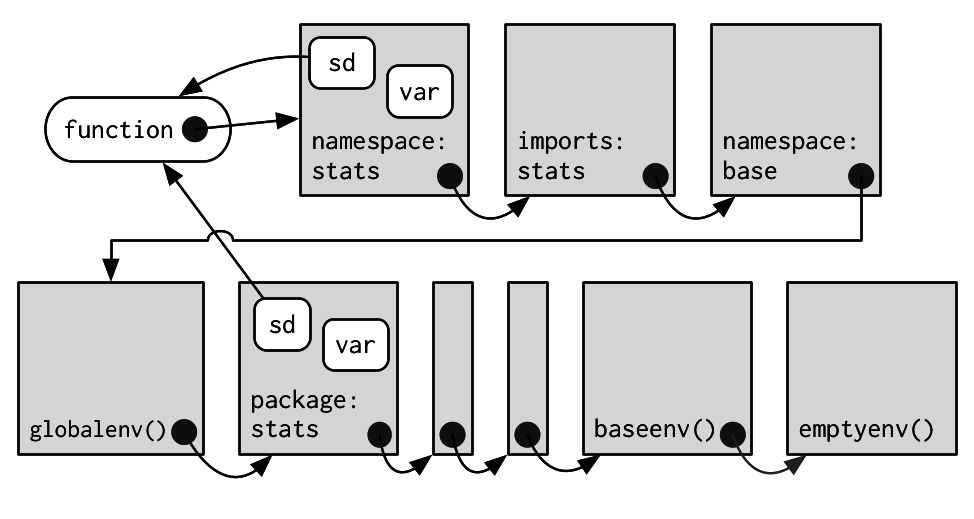
\includegraphics[scale=0.90]{figures/namespace}
			\caption{Package namespace}
			\label{fig:pkgns}
		\end{figure}
	\end{center}
\end{frame}

\begin{frame}
	\frametitle{Which are good packages}
	\centerline{Examine the package}
	\begin{center}
		\begin{enumerate}
			\item Who?			
			\item When updated?			
			\item In development?
		\end{enumerate}
	\end{center}
\end{frame}

%------------------------------------------------
\section{Git and GitHub} 
%------------------------------------------------

\begin{frame}
	\frametitle{What is Version control?}
	\begin{center}
	Video!! \\
	\href{https://vimeo.com/41027679}{Version Control}
	\end{center}
\end{frame}

\begin{frame}
	\frametitle{Why version control?}
	\begin{center}
		\begin{enumerate}
			\item Collaboration
			\item Storing versions (properly)
			\item Restoring versions
			\item Understanding what happens
			\item Backup
		\end{enumerate}
	\end{center}
\end{frame}

\begin{frame}
	\frametitle{Why git?}
	\begin{center}
		\begin{enumerate}
			\item Simple to use
			\item Distributed
			\item Fast
			\item Common in practice
			\item R packages uses github
			\item Integrated with R-Studio
		\end{enumerate}
	\end{center}
\end{frame}

\begin{frame}
	\frametitle{Why git?}
	\begin{center}
		\begin{enumerate}
			\item Simple to use
			\item Distributed
			\item Fast
			\item Common in practice
			\item R packages uses github
			\item Integrated with R-Studio
		\end{enumerate}
	\end{center}
	Created by Linus Torvalds! ;)
\end{frame}

\begin{frame}
	\frametitle{Basic git}
	\begin{center}
		\begin{figure}[!ht]
			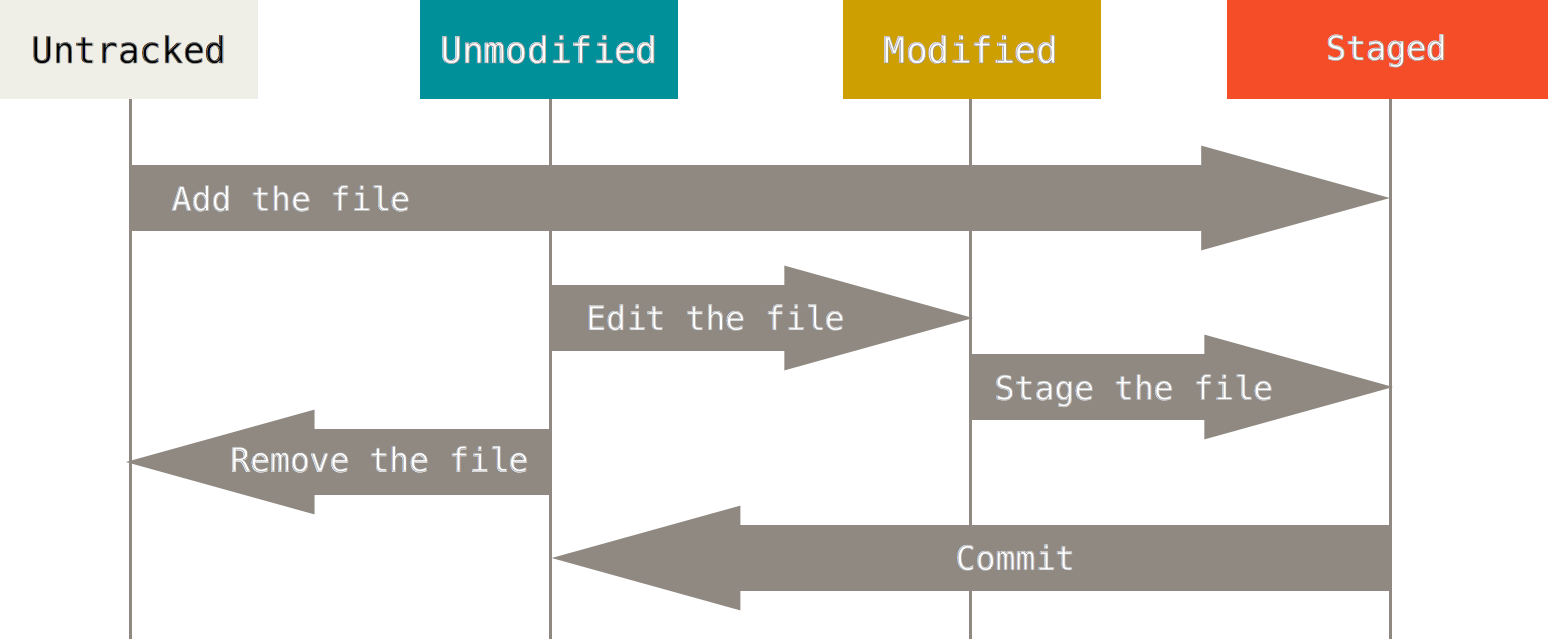
\includegraphics[scale=0.20]{figures/git-lifecycle}
			\caption{File life cycle}
			\label{fig:pkgns}
		\end{figure}
	\end{center}
\end{frame}

\begin{frame}
	\frametitle{GitHub}
	\begin{enumerate}
		\item Remote (push/pull)
		\item Barebone homepage (using md)
		\item Collaborations
		\item Issue tracker / Wiki / discussions
	\end{enumerate}
	
	Free for public repos \\
	Private repos cost \\
	Student accounts \\
\end{frame}

%------------------------------------------------
\section{Creating R packages} 
%------------------------------------------------

\begin{frame}
	\frametitle{Why part of the course?}
	Writing performant code (best practice) \\
	The way to collaborate (R ecosystem) \\
	Combine code, data and analysis \\
	Easy to distribute and reuse (public api) \\~\\
	
	Learn how to reuse code from other packages
\end{frame}

\begin{frame}
	\frametitle{Package structure}
\end{frame}

\begin{frame}
	\frametitle{Package structure}
	\texttt{DESCRIPTION}
\end{frame}

\begin{frame}
	\frametitle{Package structure}
	\texttt{DESCRIPTION} \\
	\texttt{NAMESPACE}
\end{frame}

\begin{frame}
	\frametitle{Package structure}
	\texttt{DESCRIPTION} \\
	\texttt{NAMESPACE} \\
	\texttt{R/}
\end{frame}

\begin{frame}
	\frametitle{Package structure}
	\texttt{DESCRIPTION} \\
	\texttt{NAMESPACE} \\
	\texttt{R/} \\
	\texttt{man/}
\end{frame}

\begin{frame}
	\frametitle{Package structure}
	\texttt{DESCRIPTION} \\
	\texttt{NAMESPACE} \\
	\texttt{R/} \\
	\texttt{man/} \\
	\texttt{vignette/}
\end{frame}

\begin{frame}
	\frametitle{Package structure}
	\texttt{DESCRIPTION} \\
	\texttt{NAMESPACE} \\
	\texttt{R/} \\
	\texttt{man/} \\
	\texttt{vignette/} \\
	\texttt{tests/} 
\end{frame}

\begin{frame}
	\frametitle{Package structure}
	\texttt{DESCRIPTION} \\
	\texttt{NAMESPACE} \\
	\texttt{R/} \\
	\texttt{man/} \\
	\texttt{vignette/} \\
	\texttt{tests/} \\
	\texttt{data/} 
\end{frame}

\begin{frame}
	\frametitle{Package structure}
	\texttt{DESCRIPTION} \\
	\texttt{NAMESPACE} \\
	\texttt{R/} \\
	\texttt{man/} \\
	\texttt{vignette/} \\
	\texttt{tests/} \\
	\texttt{data/} \\
	\texttt{scr/} 
\end{frame}

\begin{frame}
	\frametitle{Package structure}
	\texttt{DESCRIPTION} \\
	\texttt{NAMESPACE} \\
	\texttt{R/} \\
	\texttt{man/} \\
	\texttt{vignette/} \\
	\texttt{tests/} \\
	\texttt{data/} \\
	\texttt{scr/} \\
	\texttt{inst/} 
\end{frame}

%------------------------------------------------
\section{Documentation with ROxygen} 
%------------------------------------------------

\begin{frame}
	\frametitle{Why roxygen2?}
	\begin{enumerate}
		\item Performant code (docs close to code)
		\item Automatically generates all man files
		\item Simple to use
		\item Handles NAMESPACE
		\item Similar to JavaDoc and DOxygen
	\end{enumerate}
\end{frame}

\begin{frame}
	\frametitle{roxygen2 syntax}
	\centerline{[example]}
	\centerline{}
	\centerline{\href{https://github.com/rOpenGov/sweidnumbr}{sweidnumbr}}

	\centerline{Full support in R-Studio}
\end{frame}

%------------------------------------------------
\section{Unit testing with testthat} 
%------------------------------------------------

\begin{frame}
	\frametitle{Why unit testing?}
	Fewer bugs \\
	Better code structure \\
	Faster restarts \\
	Robust code - correct a bug only once \\~\\
	
	A must in complicated projects!
\end{frame}

\begin{frame}
	\frametitle{Types of testing}
	\begin{enumerate}
		\item White box testing
		\item Black box testing
		\item Probabilistic testing
	\end{enumerate}
\end{frame}

\begin{frame}
	\frametitle{testthat}
	\centerline{Unit testing framework for R}
	\centerline{Integrated with R-Studio}
	\centerline{}
	\centerline{[example]}
	\centerline{}
	\centerline{\href{https://github.com/rOpenGov/sweidnumbr/tree/master/tests}
		{sweidnumbr testsuite}}
\end{frame}

%------------------------------------------------
\section{R-Studio debugger} 
%------------------------------------------------

\begin{frame}
	\frametitle{Introduction to Debugging in R}
	\begin{center}
		Another Video!! \\
		\href{https://vimeo.com/99375765}{Debugging in R}
	\end{center}
\end{frame}


\begin{frame}
\Huge{\centerline{The End... for today.}}
\Huge{\centerline{Questions?}}
\Huge{\centerline{See you next time!}}
\end{frame}

%----------------------------------------------------------------------------------------

\end{document} 